\documentclass[12pt]{book}
\usepackage[utf8]{inputenc}
\usepackage{xskak}
\usepackage{amsfonts}
\usepackage{amsmath}
\usepackage{amsthm}
\usepackage{chessboard}
\usepackage[margin=1in]{geometry}
\usepackage{longtable}
\usepackage{booktabs}
\usepackage{hyperref}
\usepackage{float}
\usepackage{graphicx}

% Custom colors for move quality
\definecolor{brilliantcolor}{RGB}{0, 150, 150}
\definecolor{excellentcolor}{RGB}{0, 128, 0}
\definecolor{goodcolor}{RGB}{64, 160, 64}
\definecolor{inaccuracycolor}{RGB}{200, 180, 0}
\definecolor{mistakecolor}{RGB}{220, 120, 0}
\definecolor{blundercolor}{RGB}{200, 0, 0}

\newcommand{\FEN}{\texttt{FEN}}
\def\qqq{\mathbb{Q}}
\def\rrr{\mathbb{R}}
\def\zzz{\mathbb{Z}}

\newtheorem{example}{Example}[section]

\title{Chess Game Analyzer,\\
an introduction}
\author{David Joyner}
\date{2026-10-18}

\begin{document}
\maketitle

\tableofcontents

\newpage


\chapter*{Preface}

This is a guide to using a program I wrote to
analyze chess games you input (as a pgn file on your computer)
called the {\it chess game analyzer}, or {\it CGA} \cite{CGA26}.
The program uses other chess programs to output a
math-dense LaTeX file, called a
{\it Quantitative-Analytic Report on Chess} (or QARC),
where the results from those other programs are collected
in a human-readable format. Full disclosure: For creating CGA,
I did get a lot of help from AI: {\tt Gemini} (Google) for
chess-theoretic questions, {\tt ChatGPT} (OpenAI) for outline ideas,
and {\tt Claude} (Anthropic) for Python questions.

The CGA is a Python module providing
an advanced chess analysis pipeline that goes beyond piece
evaluations. It combines {\tt Stockfish} engine analysis with
``home-made'' positional metrics to generate quantitative
LaTeX reports on chess games, machine-readable data, and
win-prediction metrics.
In addition to generating educational content, it collects
useful game data into tables, and computes
an experimental ``Fireteam Index'' (or FTI, defined below).
As we will see below, the FTI is a family of metrics inspired by
the medieval board game rithmomachia \cite{Ri25} to measure
sustained positional dominance.

In fact, all this, the CGA module and related
programs\footnote{For instance, CGA has an add-on that creates
animated gifs of games, but such add-ons will be discussed separately.},
was inspired by the ``territorial'' approach that proper
victories take in rithmomachia. Can such an approach be helpful in
chess analysis? That question is the main motivation for this work, and
chapter~\ref{chap:testing-fti} gives a partial answer: some rithmomachia
principles help with chess and some do not.

Another goal was to create ``Prediction Algorithms'' for chess games
in the hope of predicting a win during live play.
Of course, that is impossible in general, but the question remains:
what can be done,
provided we allow some (not too many) inaccuracies?
To address this, CGA implements three algorithms that use the FTI to
predict game outcomes:

\begin{itemize}
\item
  {\tt Per-Ply}.
 \begin{itemize}
 \item
  Examines FTI at each ply (=half-move) after ply 16.
 \item
   Predicts {\it win} if FTI $> \epsilon$ (default $\epsilon = 0.2$)
   for 10 consecutive plies.
 \item
  Added plus: Captures sudden, decisive advantages.
 \end{itemize}
\item
  {\tt Windowed}
 \begin{itemize}
 \item
 This is a ``smoothed'' version of {\tt Per-Ply}.
 \item
  Computes a 10-ply rolling average of FTI, FTI$_{10}$ say.
 \item
   Applies the same streak detection to smoothed values:
   Predicts {\it win} if FTI$_{10} > \epsilon$ 
   for 10 consecutive plies.
 \item
  Filters out tactical noise; captures sustained trends.
 \end{itemize}
\item
  {\tt Balance} 
 \begin{itemize}
 \item
 Counts plies where FTI $> \epsilon$ versus FTI $<- \epsilon$
 \item
 Measures volatility $V$ (the number of times the FTI switches between
 favoring one side and favoring the other)
 \item
   Computes confidence = $|B_n|\cdot \max(0,\, 1 - V/V_{\rm thr})$,
   where $V_{\rm thr}$ is $0.2$ times the number of plies considered
\item   
  Predicts {\it draw} if confidence $<0.15$; otherwise {\it win/loss}
  (that is, not a draw).
\item
  Best at detecting drawn games and balanced struggles
 \end{itemize}
 \end{itemize}

\noindent
As chapter~\ref{chap:testing-fti} explains, on the games tested so far these
algorithms do not predict results better than simple baselines, such as
always predicting the more common result, or the same rule applied to
{\tt Stockfish}'s evaluation.

The example games are well-known and well-analyzed, so you can
compare CGA analysis here with the GM analysis published already
in books, or blogs or on youtube.
The first one is a World Correspondence Chess game played in 1965,
Estrin-Berliner, \S \ref{sec:estrin-berliner_1965}.
The second is Game 6 of the World Chess Championship match
Carlsen-Caruana in London, Nov. 2018, \S \ref{sec:carlsen-caruana_game6-2018}.

You don't need to know how to use {\tt Stockfish} or {\tt Python}
in order to run the CGA programs. However, you do need to know how to
install them on your computer if they aren't already.
Installation help and the syntax for using CGA is presented
in detail in the appendix,
ch. \ref{appendix:cga-readme}. Don't worry about the syntax or
installing software yet. First, let's learn a little more
about the CGA module.


\chapter{Introduction}

As mentioned,
detailed reference for the CGA module is given in an appendix,
ch. \ref{appendix:cga-readme}.
However, the basic idea is that the CGA module takes a pgn file as input.
The output consists of a latex report which contains the following
information about the game (or games) in the pgn file.

\begin{itemize}
\item  
Move-by-move positional analysis with Space, Mobility, King Safety, and
Threats metrics
\item  
{\tt Stockfish} suggestions of playable alternative moves within 50 centipawns
of the best 
\item  
  Game character classification (balanced/tense/tactical/chaotic,
  one-sided/seesaw)
\item  
Brilliant sacrifice detection with sound/speculative classification
\item  
An experimental Fireteam Index (FTI) combining the four metrics, in five weightings
\item
Balance and Volatility, intended to detect drawn games
\item  
Three experimental prediction algorithms (Per-Ply, Windowed, Balance) for win or draw
predictions, with held-out tests in book mode showing how well they work
\item  
Publication-quality LaTeX output with chess diagrams, plots, and methodology
\item  
Book mode for analyzing multi-game PGN files with aggregate statistics
\item  
Raw data export for downstream computational analysis

\end{itemize}

These will be explained, with examples, below.

\section{Computer chess for humans}

When a human plays chess in a given position, they use
both logic (to trace through potential moves and the
ramifications of their opponent's responses) and
experience (to restrict their analysis
to a small number of moves) in their effort to win.
The human player makes a move based on rigorous reasoning and their
previous experience with games similar to the one they are
currently playing.
They pick one that, they feel, gives them the best position no
matter what their opponent does in response. Of course,
a player will not want to lose any advantage they feel they
have in the position, whether material, or space, or mobility, or king
safety, or potential threats they can mount.
At the same time, they want their move to also
restrict their opponent's advantages in the position.

A computer plays chess using a different process.
The computer player also uses logic to sift through legal moves
for the best one. The difference is that the computer can, with the help of
a chess engine like {\tt Stockfish}, evaluate positions very rapidly
and they pick the move that both maximizes their own position
evaluation and minimizes the evaluations of each response by their opponent.
In other words, to a computer, playing chess is analogous to
solving a math problem. Can humans learn a lesson or two from how
the computer evaluates positions? Let's look more closely at this
algorithmic perspective the computer player takes.

A real-valued function $m:\FEN\to\rrr$
that takes in a position of a chess game and
returns a real number is called a {\it chess metric}.
Here, $\FEN$ simply denotes the collection of
all possible FEN positions\footnote{FEN stands for
Forsyth–Edwards Notation, a standard notation for describing a
board position, typically represented as an alphanumeric list or string,
see \cite{FEN}. Forsyth was a Scottish journalist from the
1800s while Edwards was an American computer scientist active in
computer chess from the late 1900s to early 2000s.}
and $\rrr$ is the standard notation for the set of real numbers.

One easy metric all players use is the {\it piece value metric}
for White and for Black: $PV_W({\rm fen})$ denotes the total value
of the white pieces in the position ${\rm fen}$,
and $PV_B({\rm fen})$  using the standard values for the Black pieces
in the given position.
Most players use the usual values\footnote{For more background
on the different ways to evaluate chess pieces, and there
are quite a lot of them, see 
the wikipedia article \cite{PV} and the references there
(including references to Berliner's book \cite{Be99}).} for the
pieces:

\begin{center}
\begin{tabular}{lc}
piece & value \\ \hline
king & $\infty$ \\
queen & $9$ \\
rook & $5$ \\
bishop & $3$ \\
knight & $3$ \\
pawn & $1$ \\ \hline
\end{tabular}
\end{center}

\noindent
The reader can check that, in the game's starting position,
not counting the kings, we have

\[
PV_W({\rm start}) = PV_B({\rm start}) = 39.
\]

Another example is a chess metric we'll denote
by {\tt eval}, the evaluation metric from
the chess engine {\tt Stockfish}.
This positional metric measures advantages (including piece values) in
{\it centipawns} (cp)---hundredths of a pawn.
An evaluation of $+100$ (that is, ${\tt eval}({\rm fen})>100$)
means White is ahead in the given \FEN position
by the positional equivalent of roughly one pawn. An evaluation of
$-250$ means Black has about a $2.5$ pawn advantage.

\begin{center}
\begin{tabular}{|c|c|}
Evaluation & Meaning \\ \hline
 $0$ to $\pm 50$ & Roughly equal \\
 $\pm 50$ to $\pm 150$ & Slight advantage \\
 $\pm 150$ to $\pm 300$ & Clear advantage \\
 $\pm 300$ to $\pm 500$ & Winning advantage \\
 $\pm 500+$ & Decisive advantage \\
$\pm 10000$ & Checkmate is forced \\
\end{tabular}
\end{center}

The modern {\tt Stockfish} versions primarily use NNUE (neural network)
evaluation to compute {\tt eval}. Unfortunately, that metric is a bit of
a black box. It appears to be impossible, or at least very impractical, to
directly extract from the modern {\tt Stockfish} other,
more ``territorial'' metrics such as Space.

Let's dive into that topic next.


\section{The positional metrics}

The {\tt Stockfish} evaluation {\tt eval} tells the story, metrics explain why.

As mentioned,
the modern {\tt Stockfish} {\tt eval} is a bit of a black box.

Given a chess position, how do we think of it from a territorial
perspective? These natural questions arise:

\begin{itemize}
\item
How do we compute the ``space'' controlled by a given side?

\item
How do we compute the ``mobility'' of pieces in the position?

\item
How do we compute the safety of the king?
This is, once it's defined, a defensive metric.

\item
How do we compute the ``threats'' one side has against their opponent?
Conversely, once it's defined, this is an offensive metric.
\end{itemize}

The four metrics
Space/Mobility/King Safety/Threats use the Python module
{\tt python-chess} to parse the position and then Python to directly
compute the metrics based on reasonable
formulas\footnote{For details on {\tt python-chess} and the
formulas for the metrics (Space, Mobility, and so on),
please see the following subsections or the
appendix, chapter \ref{appendix:cga-readme}.}.
These formulas are designed to address these questions.

\subsection{Data model and metric plots}

Raw positional data fields are printed at the bottom of
the \LaTeX{} QARC file, after \verb|\end{document}|, so they do not appear in the
compiled PDF. CGA uses this data to plot various chess metrics.

The FTI plots come in two versions, Per-ply and Windowed.

\begin{itemize}
\item
Per-ply: Looks for 10 consecutive positions where one side dominates
(FTI $> 0.20$). 
\item
Windowed/Smoothed: Uses a 10-ply rolling average to filter out tactical noise.
\end{itemize}

\subsection{Space}

``How much `room' do your pawns give your pieces to move in the center?''

Space evaluation counts squares in the center (files c--f, ranks 2--4 for White, 5--7 for Black) that are:
\begin{enumerate}
\item Attacked by at least one friendly pawn, {\it and}
\item Not occupied by any enemy piece
\end{enumerate}

The count is divided by 10, so Space ranges from $0$ to $1.2$
(there are 12 such squares per side); typical values are $0.1$ to $0.7$.

Space is a middlegame metric --- it becomes near-meaningless in endgames when
most pieces are traded.

\subsection{Mobility}

``How many useful squares can your pieces actually land on? (More squares = more power)''


Mobility adds $0.1$ for every square attacked by one of your pieces
(pawns included, the king excluded) that is {\it not} attacked by an enemy pawn.
A square attacked by two of your pieces counts twice, and squares occupied
by your own pieces count too, so Mobility rewards coordination as well as
freedom of movement. All piece types are weighted equally.
(QARC reports made before October 2026 show half of this value in their
tables and plots, because of a since-fixed bug; see the appendix.)

Mobility tracks piece activity. Watch it climb during development and converge as
long-range pieces (bishops, rooks, queens) are traded off.
  
\subsection{King Safety}

``How well is your King shielded by pawns, and how many nearby squares does the enemy attack?''

King safety combines two factors:
\begin{itemize}
\item \textbf{Pawn shield}: $+0.5$ for each friendly pawn on the 2nd rank
  (7th rank for Black) on the king's file or an adjacent file
\item \textbf{Attacked squares near the king}: $-0.2$ for each square within
  two squares of the king (a $5\times 5$ box) that an enemy piece attacks
\end{itemize}

King Safety can be positive and negative. Negative values in the middlegame mean danger. Negative values in the endgame can mean active, fighting kings.

\subsection{Threats}

``Are you hanging pieces, or are your small pieces attacking the opponent's big
pieces?''

Threat evaluation considers:
\begin{itemize}
\item Hanging pieces (attacked but not defended)
\item Pieces attacked by lower-value pieces (for example, a knight attacking a rook)
\item Attacks on the squares around the enemy king
\item Safe checks available
\item Weak squares (holes) in the enemy pawn structure
\end{itemize}

Threats measures potential piece captures. High threat values show tension;
when they drop sharply after exchanges, material or positional concessions
have been made.


\begin{example}
For example, the $-328$cp blunder at move 15 in \S \ref{sec:estrin-berliner-15Be2}
below shows what happened but the Mobility and Threats changes in moves 8-14
show why the position was ripe for sharp play from both sides.
\end{example}

\subsection{The Fireteam Index (experimental)}

This is a weighted sum of the differences (player minus opponent) of the four metrics above.

The Fireteam Index is a composite metric inspired by the ancient mathematical
board game {rithmomachia}, where a ``progression victory'' is achieved when a
coordinated group of pieces (a ``fireteam'') establishes control deep in enemy
territory \cite{Ri25}. Similarly, in chess, sustained positional dominance
across multiple factors often precedes victory.

CGA provides five weightings of the FTI, named for the kind of play they
emphasize (see the appendix). The original hope was that these weightings would
act as \emph{signatures} of different playing styles, and that a player who keeps
the FTI positive for long enough is on the way to winning.
Chapter~\ref{chap:testing-fti} tests both ideas; on the games tested so far,
neither holds up.



\subsection{Balance}

Balance is the key draw-detection metric. It combines:

\begin{itemize}
\item
Normalized Balance ($B_n$): the number of plies with FTI $> \epsilon$, minus
the number with FTI $< -\epsilon$, divided by the number of plies considered
\item
Volatility (V): How often the advantage changed hands
\item
Confidence (C): $C=|B_n|\cdot \max(0,\, 1 - V/V_{\rm thr})$, where $V_{\rm thr}$ is
$0.2$ times the number of plies considered.
\end{itemize}

The idea is that
if the positional metrics are roughly equal for most of the game
then neither side dominated the Space/Mobility/Threats picture consistently.
Similarly, high volatility means the advantage kept changing hands
during the course of the game. The {\it Balance algorithm} will predict
the game ends in a draw if $C < 0.15$; otherwise it predicts a win
for the side favored by $B_n$.
This data is part of the QARC output.

\chapter{Examples}

The first example game, ironically, was won by
Hans Berliner, a highly respected computer pioneer and computer science
researcher.

\section{Estrin-Berliner, 1965}
\label{sec:estrin-berliner_1965}
        
This is a popular game for commentary and analysis.
The point here is not to try to provide a summary of the
analysis of others but to report on what CGA says about
these games.

The QARC file on the game Estrin vs. Berliner (1965) describes
it as a ``chaotic seesaw battle,''
where the advantage changed hands multiple times \cite{Be65}.
 We'll walk you through this game using the provided metrics, you can use them
to explain the dynamics of the positional components (Space, Mobility, King Safety, and Threats).

White, played by the Russian chess player Yakov Estrin, took joint first place in the
USSR Correspondence Championship
a few years earlier, in 1962.
Estrin is best known for being the seventh ICCF World Champion a few
years later, in 1972–1976.

Black, played by American Hans Berliner, was also a well-known chess player.
Here is a quotation from Dunne's remembrance article for
Hans Berliner written for {\bf Chess Life} \cite{Du17}:

\begin{quotation}
The finals of the Fifth World Correspondence Chess Championship
produced a score of $14-2$, $12$ wins and four draws, a three point margin
over the second place finisher, a spread unmatched in World Championship
play. In that final, Hans also played what is widely regarded as
the greatest correspondence game ever played, and listed in Andy Soltis’
book {\bf The 100 Best Chess Games of the 20th Century} as the top game of
that tumultuous century. It is a game that has resisted major
improvement on Black’s part for over half a century.
\end{quotation}

In fact, that last statement of Dunne's is, thanks to progress in
chess engines such as {\tt Stockfish}, no longer completely true.
However, we aren't going down that rabbit hole in this guide.

\subsection{Opening phase (Moves 1–5): The Two Knights Defense}

With that background out of the way, let's see what the CGA
had to say about this game.

\vskip .1in
\noindent
{\bf 
1.e4 e5 2.Nf3 Nc6 3.Bc4 Nf6 4.Ng5 d5 5.exd5
}

\vskip .1in
\noindent
This is the famous Two Knights Defense with the Fried Liver Attack.
Estrin plays 4.Ng5,
immediately creating tension. Let's see how the metrics capture this.

Notice how Space stays roughly equal, between 0.30 and 0.40 for both sides, through move 9.
Space measures control of central squares backed by your pawns---essentially,
how much room your pieces have to maneuver.
After

\vskip .1in
\noindent
{\bf 
5.exd5
}

\vskip .1in
\noindent
White captures a pawn but Black will strike back. Watch what happens after
5...b5---the Ulvestad Variation.
The usual move in this position is 5. ... Na5.

%\begin{center}
\begin{figure}[h!]
\begin{minipage}{\textwidth}
\begin{center}
%\begin{tabular}{c}
%\hspace{4.0 cm}
  %\vspace{1.0 cm}
\chessboard[setfen=r1bqkb1r/p1p2ppp/2n2n2/1p1Pp1N1/2B5/8/PPPP1PPP/RNBQK2R w KQkq - 0 6]  
%\includegraphics[height=7cm,width=7cm]{berliner-game7-position1-after5-b5.png}
\end{center}
%\\
\begin{center}
%\hspace{4.0 cm}
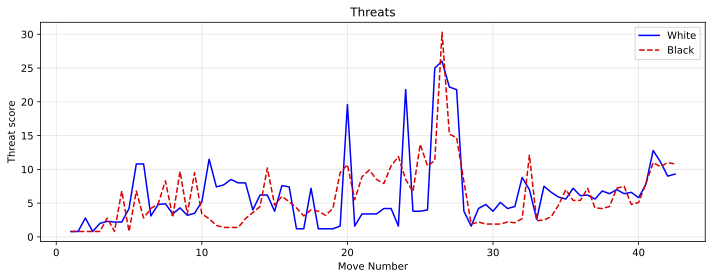
\includegraphics[height=7cm,width=12cm]{berliner-game7-threats-metric.png}
%\end{tabular}
\end{center}
\end{minipage}
\caption{(top) Position after 5 ... b5 in Estrin-Berliner (1965). (bottom) The Threats metric for that game. }
\label{fig:estrin-berliner-position1}
\end{figure}
%\end{center}

Data at ply 10/move 5:
%
%\begin{itemize}
%\item  
%Space: W 0.40, B 0.30
%\item  
%Mobility: W 4.40, B 5.10
%\item  
%King Safety: W 1.00, B -0.10
%\item  
%Threats: W 10.80, B 6.80
%\item  
Eval: +0.55
%\end{itemize}

Look at the Threats metric---White's threats spike to 10.80 because the b5-pawn is hanging.
But if you compare Black's Mobility to White's, you see
Berliner is accepting material deficit for piece activity.


\subsection{The critical opening battle (Moves 6–15)}
\label{sec:estrin-berliner-15Be2}

\vskip .1in
\noindent
{\bf
6. Bf1 Nd4 7. c3! Nxd5! 8. Ne4 Qh4?
}

\vskip .1in
\noindent
From the game's annotation by {\tt Stockfish}, both 8 ... Nc6 and 8 ... Ne6 are preferred.

\vskip .1in
\noindent
{\bf
9. Ng3! Bg4
}

\vskip .1in
\noindent
This time {\tt Stockfish} has no objection to Black's move.

\begin{center}
\begin{figure}[h!]
\begin{minipage}{\textwidth}
\begin{center}
%\begin{tabular}{c}
%\hspace{4.0 cm}
  %\vspace{1.0 cm}
\chessboard[setfen=r3kb1r/p1p2ppp/8/1p1np3/3n2bq/2P3N1/PP1P1PPP/RNBQKB1R w KQkq - 4 10]  
%\includegraphics[height=7cm,width=7cm]{berliner-game7-position2-after9-Bg4.png}
\end{center}
%\\
\begin{center}
%\hspace{4.0 cm}
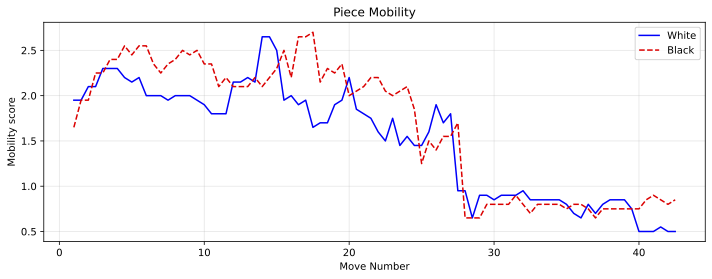
\includegraphics[height=7cm,width=12cm]{berliner-game7-mobility-metric.png}
%\end{tabular}
\end{center}
\end{minipage}
\caption{(top) Position after 9 ... Bg4 in Estrin-Berliner (1965). (bottom) The Mobility metric for that game. }
\label{fig:estrin-berliner-position2}
\end{figure}
\end{center}

Data at ply 18/move 9:

%\begin{itemize}
%\item  
%Space: W 0.30, B 0.30
%\item  
%Mobility: W 3.90, B 5.00
%\item  
%King Safety: W -0.40, B 0.50
%\item  
%Threats: W 3.50, B 9.50
%\item  
Eval: +0.99
%\end{itemize}

The game goes on (see \cite{Be65}):

\vskip .1in
\noindent
{\bf
10. f3 e4??
}

\vskip .1in
\noindent
Black loses 139cp. {\tt Stockfish} recommends 10...Bd7 instead.

\vskip .1in
\noindent
{\bf
11. cxd4 Bd6 12. Bxb5+? Kd8?! 13. O-O exf3! 14. Rxf3! Rb8!
}

\vskip .1in
\noindent
{\tt Stockfish} prefers 12. Qe2 to 12. Bxb5+. The position after 14...Rb8 is a crucial one.


\subsection{The blunder}

With threats from both sides, the next move is important.

\vskip .1in
\noindent
{\bf
15. Be2??
}

\vskip .1in
\noindent
{\it Looks} good but, in fact, some commentators say
this natural-looking move is the move that lost the game.
{\tt Stockfish} recommends 15. Bf1 instead; 15. Be2 loses about 330 centipawns.


\begin{center}
\begin{figure}[h!]
\begin{minipage}{\textwidth}
\begin{center}
%\begin{tabular}{c}
%\hspace{4.0 cm}
%\vspace{1.0 cm}
\chessboard[setfen=1r1k3r/p1p2ppp/3b4/3n4/3P2bq/5RN1/PP1PB1PP/RNBQ2K1 b - - 2 15]
%\includegraphics[height=7cm,width=7cm]{berliner-game7-position3-after15Be2.png}
%\end{center}
%\\
%\begin{center}
%\hspace{4.0 cm}
%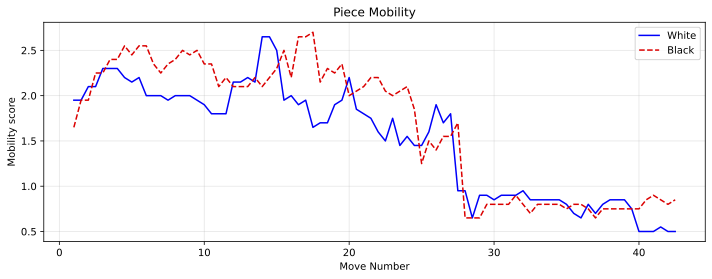
\includegraphics[height=7cm,width=12cm]{berliner-game7-mobility-metric.png}
%\end{tabular}
\end{center}
\end{minipage}
\caption{Position after 15 Be2 in Estrin-Berliner (1965).}
\label{fig:estrin-berliner-position3}
\end{figure}
\end{center}

Data at ply 29/move 15:

%\begin{itemize}
%\item  
%Space: W .30, B 0.30
%\item  
%Mobility: W 5.00, B 4.60
%\item  
%King Safety: W 0.00, B 0.10
%\item  
%Threats: W 3.80, B 4.70
%\item  
Eval: -1.57
%\end{itemize}

\subsection{The tactical middlegame (Moves 15–28)}

The game continues:

\vskip .1in
\noindent
{\bf
  16. Bxf3! Qxd4+?
}
\vskip .1in

\noindent
{\tt Stockfish} preferred instead 16... Re8.

\vskip .1in
\noindent
{\bf
17. Kh1! Bxg3! 18. hxg3! Rb6 19. d3! Ne3 20. Bxe3 Qxe3! 21. Bg4 h5! 22. Bh3! g5
23. Nd2 g4 24. Nc4! Qxg3 25. Nxb6 gxh3 26. Qf3 hxg2+ 27. Qxg2! Qxg2+!
}

\vskip .1in
\noindent
The queens are trading off now.

\subsection{The endgame, initial phase (Moves 28–34)}

Without long-range pieces, the Mobility metric drops.
We enter a new phase of the endgame.

\vskip .1in
\noindent
{\bf
28. Kxg2! cxb6 29. Rf1 Ke7 30. Re1+ Kd6 31. Rf1 Rc8?
}

\vskip .1in
\noindent
{\tt Stockfish} recommends 31...Ke6 or 31...Ke7 instead.

\begin{center}
\begin{figure}[h!]
\begin{minipage}{\textwidth}
\begin{center}
%\begin{tabular}{c}
%\hspace{4.0 cm}
%\vspace{1.0 cm}
\chessboard[setfen=2r5/p4p2/1p1k4/7p/8/3P4/PP4K1/5R2 w - - 6 32]
%\includegraphics[height=7cm,width=7cm]{berliner-game7-position4-after31-Rc8.png}
\end{center}
%\\
\begin{center}
%\hspace{4.0 cm}
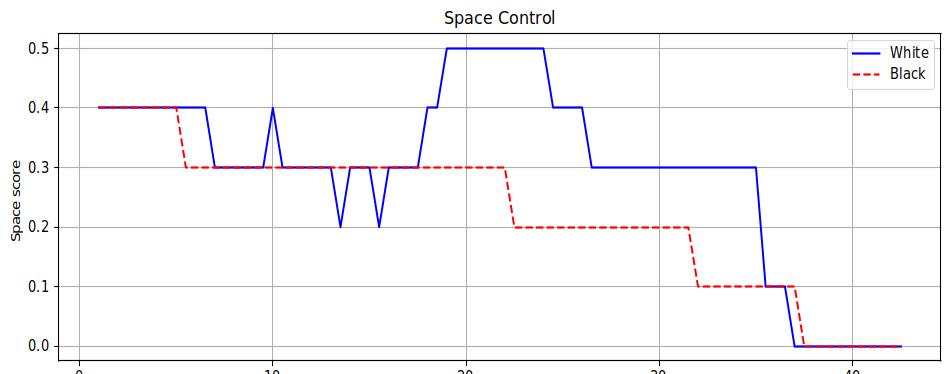
\includegraphics[height=6cm,width=12cm]{berliner-game7-space-metric.png}
%\end{tabular}
\end{center}
\end{minipage}
\caption{(top) Position after 31 ... Rc8? in Estrin-Berliner (1965). (bottom) The Space metric for that game. }
\label{fig:estrin-berliner-position4}
\end{figure}
\end{center}


Data at ply 62/move 31:

%\begin{itemize}
%\item  
%Space: W 0.30, B 0.20
%\item  
%Mobility: W 1.80, B 1.80
%\item  
%King Safety: W -0.20, B -1.20
%\item  
%Threats: W 4.50, B 2.10
%\item  
Eval: -1.28
%\end{itemize}

\vskip .1in
\noindent
{\bf
32. Rxf7 Rc7 33. Rf2?
}

\vskip .1in
\noindent
{\tt Stockfish} suggests 33. Rf5 instead.


\vskip .1in
\noindent
{\bf
33...Ke5 34. a4??
}

\vskip .1in
\noindent
This is a more serious error, but not of the same magnitude as 15 Be2??.
With 34. a4??, {\tt eval} drops from $-1.90$ to $-3.52$.
Here, {\tt Stockfish} recommends instead Rf8.

\vskip .1in
\noindent
{\bf
34...Kd4! 35. a5 Kxd3
}


\subsection{The final phase (Moves 35–42)}

The final moves of the game.

\vskip .1in
\noindent
{\bf
36. Rf3+! Kc2! 37. b4?! b5! 38. a6? Rc4?! 39. Rf7 Rxb4! 40. Rb7? Rg4+! 41. Kf3
}

\vskip .1in
\noindent
{\tt Stockfish} flags 38. a6? (38. Rf5 was better) and 40. Rb7? (40. Rxa7 was better).

\vskip .1in
\noindent
{\bf 
41...b4! 42. Rxa7 b3! 0-1
}

\vskip .1in


\subsection{FTI summary}

Recall that the FTI is a weighted sum of the differences
(player minus opponent) in the four positional metrics,
Space (S), Mobility (M), King Safety (KS), and Threats (T):

\[
FTI = w_S\,\Delta S + w_M\,\Delta M + w_{KS}\,\Delta KS + w_T\,\Delta T',
\]
where $T' = T/20$ (see the appendix).
Think of the FTI as a coordinated pressure gauge.
Figure~\ref{fig:estrin-berliner-1965-FTI1} shows FTI1, which weights the four
metrics equally.

\begin{figure}[H]
\begin{center}
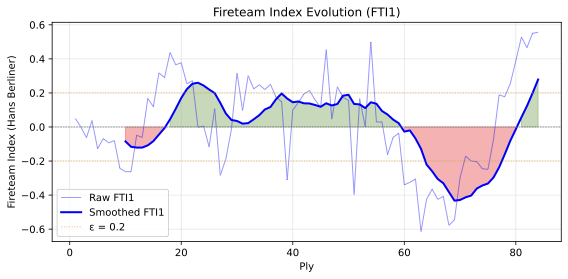
\includegraphics[height=7cm,width=12cm]{estrin-berliner-1965-FTI1.png}
\end{center}
\caption{Fireteam index FTI1 (equal weights) for Estrin-Berliner, 1965.}
\label{fig:estrin-berliner-1965-FTI1}
\end{figure}

The game was so volatile that the FTI swings back and forth.
With the current version of CGA, the Per-ply rule (dominance for 10 consecutive
plies) does not predict Black's win with any of the five weightings; the
Windowed rule does with FTI1 and FTI4.
More importantly, across all 16 of Berliner's games in this championship, the
tests in chapter~\ref{chap:testing-fti} find no evidence that the FTI predicts
results better than simple baselines, or that any weighting of it describes
Berliner's style.

\section{Carlsen-Caruana, Game 6, 2018}
\label{sec:carlsen-caruana_game6-2018}

At this point in the match, the players were tied
2.5-2.5, with 5 draws in a row. This game was another draw but exciting nonetheless.
In fact, on move 67 it appears Caruana missed a win.

The QARC file on the $12$ games in the Carlsen-Caruana match, London
(November 2018) is available online as a pdf \cite{CC18}.
We'll walk you through this game using the provided metrics,
you can use them
to explain the dynamics of the positional components
(Space, Mobility, King Safety, and Threats).

Of course, both players are well-known.
In 2018, the 27-year-old Norwegian was the undisputed king of chess,
having held the World Championship title since 2013 and the world
No. 1 ranking since 2011.
The 26-year-old Italian-American grandmaster, in 2018, became
the first American to challenge for the undisputed world chess title since
Bobby Fischer in 1972.
At the time of their match, their Elo ratings were nearly the same.


\subsection{The early opening moves (1-4)}

Look at the plot for {\tt Stockfish}'s {\tt eval} function (see Figure \ref{fig:carlsen-caruana-position1}).


\begin{center}
\begin{figure}[h!]
\begin{minipage}{\textwidth}
\begin{center}
%\begin{tabular}{c}
%\hspace{4.0 cm}
%\vspace{1.0 cm}
%\includegraphics[height=7cm,width=7cm]{berliner-game7-position4-after31-Rc8.png}
\chessboard[setfen=rnbqkb1r/ppp2ppp/3p1n2/8/4P3/3N4/PPPP1PPP/RNBQKB1R b KQkq - 1 4]
\end{center}
%\\
\begin{center}
%\hspace{4.0 cm}
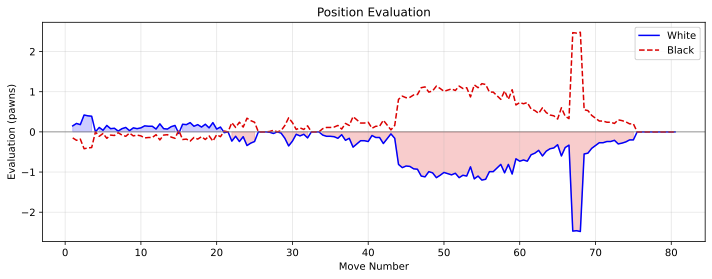
\includegraphics[height=7cm,width=12cm]{carlsen-caruana-game6-eval-metric.png}
%\end{tabular}
\end{center}
\end{minipage}
\caption{(top) Position after 4 Nd3?! in Carlsen-Caruana, Game 6 (2018). (bottom) The {\tt eval} metric for that game. }
\label{fig:carlsen-caruana-position1}
\end{figure}
\end{center}

Notice how the line hovers around zero for the first 10-15 moves,
then drifts into negative territory,
favoring Caruana. The game reaches its most critical point around
moves 67-68 where we see a
dramatic spike to about $-2.3$ pawns, a large advantage for Black.
Unfortunately for Caruana, that was followed by an equally dramatic
swing back toward zero.


\vskip .1in

\noindent
{\bf
1. e4 e5
2. Nf3 Nf6
3. Nxe5 d6
4. Nd3?!
}

\vskip .1in
\noindent
While this is part of opening theory\footnote{ECO C42:
Petrov’s Defence, Karklins-Martinovsky Variation, to be precise.},
{\tt Stockfish} marks Carlsen's move as an inaccuracy (?!).

\vskip .2in
%\begin{figure}

\noindent
{\bf Position 1: After 4. Nd3 }

\noindent
Evaluation: +0.08
%\begin{center}

%\begin{small}
%\begin{tabular}{lcc}
%\toprule
%Metric & White & Black \\
%\midrule
%Space & 0.40 & 0.60 \\
%Mobility & 4.10 & 4.10 \\
%King Safety & 1.00 & 0.50 \\
%Threats & 0.80 & 2.80 \\
%\bottomrule
%\end{tabular}
%\end{small}

%\end{center}
%\end{figure}

\vskip .2in

\newpage

\subsection{The opening phase (5-15)}

\vskip .1in

\noindent
{\bf
4 ... Nxe4
5. Qe2 Qe7
6. Nf4 Nc6
7. Nd5! Nd4!
8. Nxe7 Nxe2!
9. Nd5! Nd4!
10. Na3 Ne6!
11. f3! N4c5
12. d4! Nd7
13. c3 c6!
14. Nf4! Nb6!
15. Bd3 d5
}
% fen = r1b1kb1r/pp3ppp/1np1n3/3p4/3P1N2/N1PB1P2/PP4PP/R1B1K2R w KQkq - 0 16

\vskip .1in
\noindent
This is all part of the opening. White is given a slight advantage by {\tt Stockfish}.

Figure \ref{fig:carlsen-caruana-position3}
tells us Caruana successfully seized territorial control (Space) in the opening up to move 15.
In Figure \ref{fig:carlsen-caruana-position4}, look at how the Mobility values drop
after the unusual early queen trade on move 8.


  \vskip .1in
\noindent
{\bf Position 2: After 15. ... d5 }
\begin{center}
  \chessboard[setfen=r1b1kb1r/pp3ppp/1np1n3/3p4/3P1N2/N1PB1P2/PP4PP/R1B1K2R w KQkq - 0 16]

  \vskip .1in
  After {\bf 15. ... d5}.
\end{center}


\subsection{The early middlegame (16-25)}

The game continued:
\vskip .2in

\noindent
{\bf
16. Nc2! Bd6
17. Nxe6 Bxe6
18. Kf2! h5!
19. h4! Nc8
20. Ne3 Ne7
21. g3! c5!
22. Bc2 O-O
23. Rd1 Rfd8
24. Ng2 cxd4!
25. cxd4 Rac8
}

\vskip .1in
\noindent
This ends the early middlegame. The game is even, according to {\tt Stockfish}.

\vskip .1in
\noindent
{\bf Position 3: After 25. ... Rac8 }
\begin{center}
\begin{figure}[h!]
\begin{minipage}{\textwidth}
\begin{center}
%\begin{tabular}{c}
%\hspace{4.0 cm}
%\vspace{1.0 cm}
\chessboard[setfen=2rr2k1/pp2npp1/3bb3/3p3p/3P3P/5PP1/PPB2KN1/R1BR4 w - - 1 26]
\end{center}
%\\
\begin{center}
%\hspace{4.0 cm}
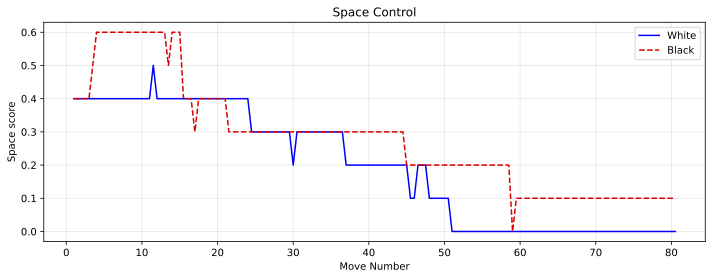
\includegraphics[height=7cm,width=12cm]{carlsen-caruana-game6-space-metric.png}
%\end{tabular}
\end{center}
\end{minipage}
\caption{(top) Position after 25 ... Rac8 in Carlsen-Caruana, Game 6 (2018). (bottom) The Space metric for that game. }
\label{fig:carlsen-caruana-position3}
\end{figure}
\end{center}

\newpage

\subsection{The later middlegame (26-33)}

The game continued:
\vskip .2in

\noindent
{\bf
26. Bb3! Nc6
27. Bf4 Na5!
28. Rdc1! Bb4
29. Bd1?! Nc4
30. b3! Na3
31. Rxc8! Rxc8!
32. Rc1! Nb5
33. Rxc8+! Bxc8!
}

% fen = 2b3k1/pp3pp1/8/1n1p3p/1b1P1B1P/1P3PP1/P4KN1/3B4 w - - 0 34

\vskip .1in

\noindent
{\bf Position 4: After 33. ... Bxc8! }
\begin{center}
\begin{figure}[h!]
\begin{minipage}{\textwidth}
\begin{center}
%\begin{tabular}{c}
%\hspace{4.0 cm}
%\vspace{1.0 cm}
\chessboard[setfen=2b3k1/pp3pp1/8/1n1p3p/1b1P1B1P/1P3PP1/P4KN1/3B4 w - - 0 34]
\end{center}
%\\
\begin{center}
%\hspace{4.0 cm}
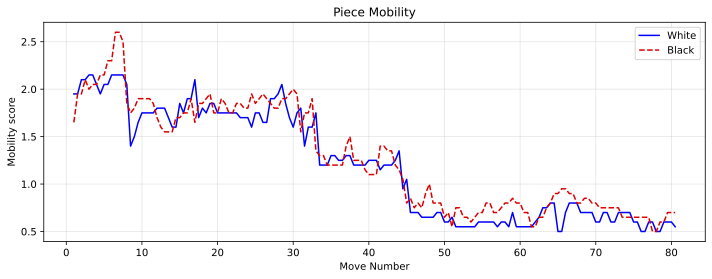
\includegraphics[height=7cm,width=12cm]{carlsen-caruana-game6-mobility-metric.png}
%\end{tabular}
\end{center}
\end{minipage}
\caption{(top) Position after 33 ... Bxc8 in Carlsen-Caruana, Game 6 (2018). (bottom) The Mobility metric for that game. }
\label{fig:carlsen-caruana-position4}
\end{figure}
\end{center}

\vskip .1in

\noindent
Note how the Mobility metric drops after these piece exchanges.

\newpage

\subsection{The early endgame (34-67)}

The game continued:
\vskip .2in

\noindent
{\bf
34. Ne3 Nc3!
35. Bc2! Ba3!
36. Bb8 a6
37. f4 Bd7
38. f5?! Bc6!
39. Bd1! Bb2
40. Bxh5 Ne4+
41. Kg2! Bxd4!
42. Bf4 Bc5!
43. Bf3! Nd2
}

\vskip .1in

\noindent
This is a very interesting move, setting in motion a long combination,
dropping piece Mobility but escalating Threats.

\newpage

\noindent
{\bf Position 5: After 43. Bf3 }
\begin{center}
\begin{figure}[H]
\begin{minipage}{\textwidth}
\begin{center}
%\begin{tabular}{c}
%\hspace{4.0 cm}
%\vspace{1.0 cm}
\chessboard[setfen=6k1/1p3pp1/p1b5/2bp1P2/4nB1P/1P2NBP1/P5K1/8 b - - 3 43]
\end{center}
%\\
\begin{center}
%\hspace{4.0 cm}
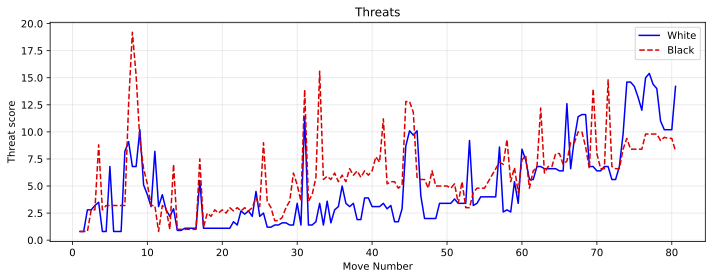
\includegraphics[height=7cm,width=12cm]{carlsen-caruana-game6-threats-metric.png}
%\end{tabular}
\end{center}
\end{minipage}
\caption{(top) Position after 43 Bf3 and before 43 ... Nd2! in Carlsen-Caruana, Game 6 (2018). (bottom) The Threats metric for that game. }
\label{fig:carlsen-caruana-position5}
\end{figure}
\end{center}


\vskip .1in
\noindent
{\bf
44. Bxd5?
}

\vskip .1in

\noindent
{\tt Stockfish} didn't like Carlsen's move and suggests considering Nf1 or Nd1 instead.

\vskip .1in

\noindent
{\bf Position 6: After 44. Bxd5}

Evaluation: -0.80

%\chessboard[setfen=6k1/1p3pp1/p1b5/2bB1P2/5B1P/1P2N1P1/P2n2K1/8 b - - 0 44]

%\begin{small}
%\begin{tabular}{lcc}
%\toprule
%Metric & White & Black \\
%\midrule
%Space & 0.20 & 0.30 \\
%Mobility  & 2.70 & 2.30 \\
%King Safety & -0.80 & 0.20 \\
%Threats & 2.90 & 5.10 \\
%\bottomrule
%\end{tabular}
%\end{small}

\vskip .1in

\noindent
The game continued:
\vskip .2in

\noindent
{\bf
44...Bxe3!
45. Bxc6! Bxf4!
46. Bxb7! Bd6
47. Bxa6 Ne4!
48. g4! Ba3!
49. Bc4 Kf8
50. g5 Nc3!
51. b4 Bxb4
52. Kf3 Na4!
53. Bb5 Nc5?!
54. a4?! f6
55. Kg4! Ne4
56. Kh5 Be1
57. Bd3?! Nd6
58. a5 Bxa5!
59. gxf6! gxf6!
60. Kg6! Bd8
61. Kh7 Nf7?!
62. Bc4! Ne5
63. Bd5! Ba5
64. h5! Bd2
65. Ba2 Nf3
66. Bd5 Nd4
67. Kg6?!
}

\vskip .1in
\noindent
{\tt Stockfish} marks this as an inaccuracy: after 67...Bg5, Black is more than two pawns ahead.

\vskip .1in
\noindent
{\bf Position 7: After 67. Kg6}

Evaluation: -1.35

\chessboard[setfen=5k2/8/5pK1/3B1P1P/3n4/8/3b4/8 b - - 6 67]

%\begin{small}
%\begin{tabular}{lcc}
%\toprule
%Metric & White & Black \\
%\midrule
%Space & 0.00 & 0.10 \\
%Mobility (MG) & 1.60 & 1.80 \\
%King Safety & -2.20 & -1.60 \\
%Threats & 9.40 & 9.00 \\
%\bottomrule
%\end{tabular}
%\end{small}

\subsection{The later endgame (67-80)}

After 67...Bg5, {\tt Stockfish} rates Black's advantage at $-2.27$, the largest of the game.

\vskip .1in

\noindent
{\bf
67...Bg5!
68. Bc4 Nf3??
}

\vskip .1in

\noindent
According to {\tt Stockfish}, this is a blunder; it recommends Bh4 instead.
According to {\tt Stockfish}, with depth=23, with this knight move Caruana missed a win.

\begin{center}
\begin{figure}[H]
\begin{minipage}{\textwidth}
\begin{center}
%\begin{tabular}{c}
%\hspace{4.0 cm}
%\vspace{1.0 cm}
\chessboard[setfen=5k2/8/5pK1/5PbP/2B5/5n2/8/8 w - - 9 69]
\end{center}
%\\
\begin{center}
%\hspace{4.0 cm}
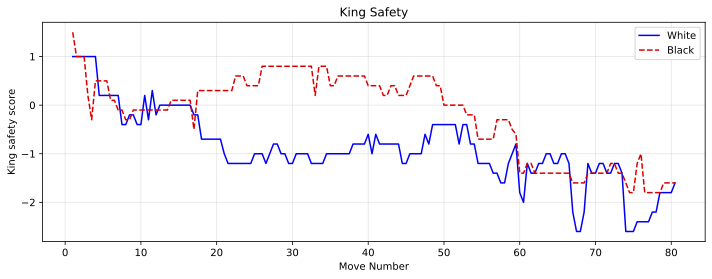
\includegraphics[height=7cm,width=12cm]{carlsen-caruana-game6-king-safety-metric.png}
%\end{tabular}
\end{center}
\end{minipage}
\caption{(top) Position after 68 ... Nf3?? (moving from d4) in Carlsen-Caruana, Game 6 (2018).  (bottom) The King Safety metric for that game. }
\label{fig:carlsen-caruana-position8}
\end{figure}
\end{center}

\vskip .1in
After 18 Kf2, the White king enters the game early instead of castling, which
here created the opportunity for Black to make more threats.
Based on Figure \ref{fig:carlsen-caruana-position8} (bottom),
note the King Safety line drops into negative territory (-0.7 to -1.2) after the opening and stays there.
On the other hand, Black's King Safety was positive from moves 18 to 50 (after 49 ... Kf8).
Since Carlsen's king was more exposed to checks and needed protection, Caruana was able to
keep stronger positional evaluations, even with equal material.

\newpage

The game concluded this way:

\vskip .1in

\noindent
{\bf
69. Kh7 Ne5
70. Bb3 Ng4
71. Bc4 Ne3!
72. Bd3! Ng4
73. Bc4 Nh6
74. Kg6 Ke7
75. Bb3! Kd6?!
76. Bc2! Ke5
77. Bd3 Kf4
78. Bc2 Ng4
79. Bb3 Ne3?!
80. h6! Bxh6!
1/2-1/2
}

\subsection{FTI summary}

Figure~\ref{fig:carlsen-caruana-2018-FTI1} shows FTI1 (equal weights) for this game.

\begin{figure}[H]
\begin{center}
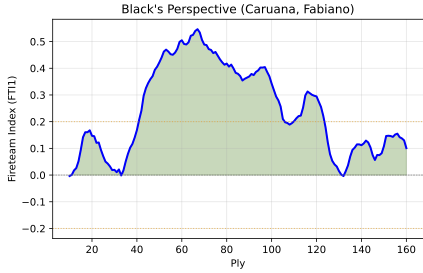
\includegraphics[height=7cm,width=12cm]{carlsen-caruana-2018-FTI1.png}
\end{center}
\caption{Fireteam index FTI1 (equal weights) for game 6 of Carlsen-Caruana, 2018.}
\label{fig:carlsen-caruana-2018-FTI1}
\end{figure}

All twelve classical games of this match were drawn, so the FTI cannot be tested
as a predictor of results on this match: there is no variation in results to
learn from. (An earlier version of this manual reported ``optimal'' weights
$(0, 0, 0, 1)$ with $R^2 = 0$ for this match; those numbers were an artifact of
fitting weights to twelve identical results.)

Chapter~\ref{chap:testing-fti} asks a different question of this match: given
several near-equal moves, do Carlsen and Caruana choose differently, as measured
by the four metrics? They do not. A model fitted to Caruana's choices predicts
Carlsen's as well as Carlsen's own model does, and vice versa.

\chapter{Testing the Fireteam Index}
\label{chap:testing-fti}

The FTI was built on a rithmomachia idea: a coordinated group of pieces
(a ``fireteam'') that establishes control deep in enemy territory, and holds
it, is on the way to victory. This chapter tests two consequences of that idea
on the games in this manual:
\begin{enumerate}
\item sustained FTI dominance predicts the result of a game, and
\item the FTI weights capture a player's style, so they could be used to
  predict the kind of move a player will choose.
\end{enumerate}
The short answer is that some rithmomachia principles help with chess and some
do not.

\section{Does sustained dominance predict the result?}

Berliner scored 12 wins and 4 draws in his 16 games of the 5th World
Correspondence Championship \cite{Be65}. Table~\ref{tab:outcome-tests}
compares the FTI prediction rules with two baselines: always predicting a
Berliner win, and the same 10-ply streak rule applied to {\tt Stockfish}'s
evaluation (Berliner more than one pawn ahead). The last row refits the
FTI weights 16 times, each time leaving one game out and predicting it.
The ``first half'' column uses only the first half of each game, which is
the useful case for prediction: by the end of a game, the evaluation nearly
shows the result. All numbers were computed with the current version of CGA
from the raw data in \cite{Be65}.

\begin{table}[H]
\begin{center}
\begin{tabular}{lcc}
\toprule
\textbf{Method} & \textbf{Whole games} & \textbf{First half only} \\
\midrule
Always predict a Berliner win & 12/16 & 12/16 \\
Streak rule on {\tt Stockfish}'s evaluation & 15/16 & 8/16 \\
FTI1 (Harmonious), Per-ply rule & 7/16 & 6/16 \\
FTI2 (Tactical), Per-ply rule & 7/16 & 6/16 \\
FTI3 (Strategic), Per-ply rule & 8/16 & 6/16 \\
FTI4 (Dynamic), Per-ply rule & 11/16 & 8/16 \\
FTI5 (Solid), Per-ply rule & 7/16 & 5/16 \\
FTI weights refit with the game held out & 13/16 & 11/15$^*$ \\
\bottomrule
\end{tabular}
\end{center}
\caption{Correct predictions of Berliner's results. $^*$One game's first half is entirely within the first 16 plies, which the FTI ignores.}
\label{tab:outcome-tests}
\end{table}

No FTI rule beats simply predicting a Berliner win every time. The FTI is
also only weakly related to the evaluation: across all positions after ply 16,
the correlation between FTI1 and {\tt Stockfish}'s evaluation is $0.28$.
For the 2018 Carlsen-Caruana match no such test is possible, because all
twelve games were drawn.

In book mode, CGA now runs the held-out test (the last row) on every
collection, in place of the ``empirically optimal weights'' that earlier
versions printed. Those weights and their $R^2$ values (for example,
$R^2 = -12.5$ for Berliner's games) were not meaningful: the fit had no
constant term, and its weights were clipped and rescaled afterwards.

\section{Do the FTI weights describe a playing style?}

Results are a poor guide to style: they mostly reflect who made fewer
mistakes. A better guide is the moves a player chooses. In many positions,
{\tt Stockfish} rates several moves as nearly equal; which one a player picks
is a matter of taste. If Berliner keeps choosing the move that raises his
Mobility over the one that gains Space, that \emph{is} his style.

\paragraph{Method.} For every position after move 8 in Berliner's 16 games
and the 12 games of the 2018 match\footnote{With the colors of the actual
games. Before October 2026, the QARC file \cite{CC18} listed Carlsen as White in
all twelve games, which was wrong for games 1, 3, 5, 8, 10, and 12; the current
version is correct.}, {\tt Stockfish}~16 (depth 14)
listed its six best moves. The \emph{candidates} are the moves within
50 centipawns of the best. That leaves 1,455 positions with a real choice,
after dropping 370 positions with only one playable move and 91 where the move
played was more than 50 centipawns worse. For each candidate, CGA computed the
change in Space, Mobility, King Safety and Threats (player minus opponent).
A standard statistical model of choices (a conditional logit) then estimates
how much each metric, and the evaluation, sways the player's choice.
Every model was tested only on games it was not fitted on.

\begin{table}[H]
\begin{center}
\begin{tabular}{lrrrr}
\toprule
\textbf{Player} & \textbf{Choices} & \textbf{Random pick} & \textbf{Eval only} & \textbf{Eval + 4 metrics} \\
\midrule
Berliner & 281 & 31\% & 60\% & 57\% \\
Berliner's opponents & 276 & 29\% & 50\% & 48\% \\
Carlsen & 459 & 22\% & 49\% & 46\% \\
Caruana & 439 & 24\% & 53\% & 49\% \\
\bottomrule
\end{tabular}
\end{center}
\caption{How often each model's most likely move was the move actually played, on held-out games.}
\label{tab:move-choice}
\end{table}

The results (Table~\ref{tab:move-choice}) are clear:
\begin{itemize}
\item Adding the four metrics to the evaluation makes the predictions slightly
  \emph{worse} for every player, so the metrics do not reveal a personal style.
\item Carlsen and Caruana cannot be told apart: a model fitted to Caruana's
  choices predicts Carlsen's as well as Carlsen's own model does, and vice versa.
\item Berliner's own model does beat his opponents' model, but only because he
  picks {\tt Stockfish}'s preferred move more often. That is playing strength,
  not style.
\end{itemize}

\section{What helps and what does not}

There is one consistent pattern, and every group in the study shares it.
Among near-equal moves, players pick the candidate that most increases their
Threats, Mobility, or King Safety a few percentage points more often than a
random choice would (Table~\ref{tab:top-choice}). Space barely matters.

\begin{table}[H]
\begin{center}
\begin{tabular}{lcc}
\toprule
\textbf{Candidate scoring highest on} & \textbf{Excess over random choice} & \textbf{90\% interval} \\
\midrule
{\tt Stockfish}'s evaluation & $+25.1$ points & $+23.0$ to $+27.4$ \\
Threats & $+6.3$ points & $+4.6$ to $+8.0$ \\
Mobility & $+4.7$ points & $+3.1$ to $+6.5$ \\
King Safety & $+4.4$ points & $+2.4$ to $+6.4$ \\
Space & $+1.7$ points & $+0.8$ to $+2.7$ \\
\bottomrule
\end{tabular}
\end{center}
\caption{How much more often than random the move played was the candidate
scoring highest on each measure, over all 1,455 choices (intervals by
resampling games).}
\label{tab:top-choice}
\end{table}

\noindent
Putting the two studies together:

\begin{itemize}
\item \textbf{Principles that help.} Coordination and activity (Mobility) and
  pressure on the enemy (Threats), the ``fireteam'' half of the rithmomachia
  idea, describe how strong players choose among equally good moves. They are
  shared by all the players studied, so they describe good chess rather than one
  player's style, and they are too weak to improve predictions once
  {\tt Stockfish}'s evaluation is known. The metric plots in the examples above
  also help explain \emph{why} a game went the way it did.
\item \textbf{Principles that do not help.} Territory as such (Space) barely
  influences the choices of strong players. Holding positional dominance as a
  winning condition (the FTI prediction rules) does not predict results better
  than simple baselines. And no weighting of the FTI acts as a signature of a
  player's style.
\end{itemize}

These are small samples (fewer than 500 choices per player), the four metrics
are simple, and the candidate moves came from a modest search depth. Better
metrics might find something these four do not, and the tests above, which CGA
now runs on every book, are the way to find out.

% =============================================================================
% Chess Game Analyzer - README Documentation
% Suitable for inclusion as an appendix in a manual
% =============================================================================

\chapter{Appendix: Chess Game Analyzer module reference}
\label{appendix:cga-readme}

This is the readme file for the CGA program \cite{CGA26} generated by {\tt Claude} (Anthropic),
with some editing by me.

\section{Overview}

The Chess Game Analyzer is a Python module for deep positional analysis of chess games using Stockfish, with comprehensive \LaTeX{} report generation and win prediction metrics.

Chess Game Analyzer goes beyond simple engine evaluation to provide interpretable positional metrics for every move of a chess game. It computes Space control, Mobility, King Safety, and Threats directly from board positions, then combines these into \textbf{Fireteam Index (FTI)} metrics that can predict game outcomes based on sustained positional advantages.

The module generates professional \LaTeX{} reports with annotated games, critical position diagrams, matplotlib plots, and detailed methodology explanations---suitable for chess study, coaching, or research.


% -----------------------------------------------------------------------------
\section{Background for Newcomers}
% -----------------------------------------------------------------------------

\subsection{What is Stockfish?}

{\tt Stockfish}\footnote{\url{https://stockfishchess.org/}} is the world's strongest open-source chess engine. It analyzes positions and calculates the best moves by searching millions of positions per second. This module uses Stockfish to evaluate positions, but computes the positional breakdown (Space, Mobility, etc.)\ directly using the {\tt python-chess} library.

\textbf{Stockfish must be installed on your system.} Download it from the
official website and note the installation path.

\subsection{What is a Centipawn?}

Chess engines measure advantages in \textbf{centipawns (cp)}---hundredths of a pawn. An evaluation of $+100$ means White is ahead by roughly one pawn's worth of material or positional compensation. An evaluation of $-250$ means Black has about a 2.5 pawn advantage.

\begin{center}
\begin{tabular}{ll}
\toprule
\textbf{Evaluation} & \textbf{Meaning} \\
\midrule
$0$ to $\pm 50$ & Roughly equal \\
$\pm 50$ to $\pm 150$ & Slight advantage \\
$\pm 150$ to $\pm 300$ & Clear advantage \\
$\pm 300$ to $\pm 500$ & Winning advantage \\
$\pm 500+$ & Decisive advantage \\
$\pm 10000$ & Checkmate is forced \\
\bottomrule
\end{tabular}
\end{center}

\subsection{Python Requirements}

The module requires:
\begin{itemize}
    \item \textbf{Python 3.8 or higher}
    \item \textbf{python-chess} (installed as {\tt chess}): The chess library that handles board representation, move generation, and PGN parsing
    \item \textbf{matplotlib} (optional): For generating plots; the module works without it using ASCII plots.
      Plots also need the file \texttt{chess\_plotting.py} in the same folder as \texttt{chess\_game\_analyzer.py}.
\end{itemize}

To install the dependencies:
\begin{verbatim}
pip install chess matplotlib
\end{verbatim}

% -----------------------------------------------------------------------------
\section{Installation}
% -----------------------------------------------------------------------------

\begin{enumerate}
    \item \textbf{Install Stockfish} from \url{https://stockfishchess.org/download/}
    
    \item \textbf{Clone the repository} \url{https://github.com/wdjoyner/chess-animator} or download \texttt{chess\_game\_analyzer.py} and \texttt{chess\_plotting.py} from it.
    Keep both files in the same folder: without \texttt{chess\_plotting.py}, reports are produced with no plots.
    
    \item \textbf{Install Python dependencies}:
\begin{verbatim}
pip install chess matplotlib
\end{verbatim}
    
    \item \textbf{Verify Stockfish path}:
\begin{verbatim}
# Linux/Mac - find where Stockfish is installed
which stockfish

# Or test directly
stockfish
\end{verbatim}
\end{enumerate}

% -----------------------------------------------------------------------------
\section{Quick Start}
% -----------------------------------------------------------------------------

\subsection{Command Line}

\begin{verbatim}
# Analyze a single game
python chess_game_analyzer.py game.pgn -o analysis.tex

# Analyze with custom Stockfish path and deeper analysis
python chess_game_analyzer.py game.pgn -o analysis.tex \
    --stockfish /usr/local/bin/stockfish \
    --depth 22 \
    --time 2.0

# Analyze multiple games as a book
python chess_game_analyzer.py tournament.pgn -o book.tex --book \
    --book-title "My Tournament Games" \
    --book-author "Your Name"
\end{verbatim}

\subsection{Python API}

\begin{verbatim}
from chess_game_analyzer import (
    EnhancedGameAnalyzer,
    EnhancedLaTeXReportGenerator,
    classify_game_character
)

# Analyze a game
with EnhancedGameAnalyzer("/usr/local/bin/stockfish", 
                          depth=20, time_limit=1.0) as analyzer:
    result = analyzer.analyze_game("game.pgn")

# Access move-by-move data
for move in result.moves:
    pos = move.positional_eval
    print(f"Move {move.ply}: {move.move_san}")
    print(f"  Space: W={pos.space_white:.2f}, B={pos.space_black:.2f}")
    print(f"  Mobility: W={pos.mobility_white:.2f}, B={pos.mobility_black:.2f}")
    print(f"  Eval: {move.eval_after/100:+.2f} pawns")

# Generate LaTeX report
latex = EnhancedLaTeXReportGenerator.generate_report(
    result,
    include_plots=True,
    include_methodology=True
)
with open("analysis.tex", "w") as f:
    f.write(latex)
\end{verbatim}

% -----------------------------------------------------------------------------
\section{Positional Metrics Explained}
% -----------------------------------------------------------------------------

\subsection{Space}

\textbf{Space} measures territorial control: central squares in your own half of the board that your pawns guard.

The computation counts squares on central files (c--f) in ranks 2--4 (for White) or 5--7 (for Black) that are:
\begin{enumerate}
    \item Attacked by at least one friendly pawn, {\it and}
    \item Not occupied by an enemy piece
\end{enumerate}

The raw count is divided by 10 to normalize the metric. Values typically range from 0.1 to 0.7.

\paragraph{Example from Estrin vs Berliner (1965), ply 20 (10...e4):}
\begin{itemize}
    \item White Space: 0.30
    \item Black Space: 0.30
\end{itemize}
At this point in a sharp Two Knights Defense, space is roughly equal, but the position is about to explode tactically.

\subsection{Mobility}

\textbf{Mobility} adds $0.1$ for every square attacked by one of your pieces
(pawns included, the king excluded) that is not attacked by an enemy pawn.
All piece types count equally, a square attacked by two of your pieces counts twice,
and squares occupied by your own pieces count too.
The metric captures piece activity and coordination.

\textbf{Note on scale.} In QARC reports made before October 2026, including the two
cited in this manual, the Mobility values in the tables and plots are half of this value,
because of a since-fixed bug. The raw data block at the end of each \LaTeX{} file
always stores the full value, and the numbers below use the full value.

\paragraph{Example from Estrin vs Berliner, ply 30 (15...Bxf3):}
\begin{itemize}
    \item White Mobility: 3.90
    \item Black Mobility: 5.00
\end{itemize}
After White's blunder 15.Be2??, Black's pieces have become significantly more active.

\subsection{King Safety}

\textbf{King Safety} combines two factors:

\begin{enumerate}
    \item \textbf{Pawn shield}: $+0.5$ for each friendly pawn on the 2nd rank (7th for Black) on the king's file or an adjacent file
    \item \textbf{Attacked squares}: $-0.2$ for each square within two squares of the king that an enemy piece attacks
\end{enumerate}

Positive values indicate a safe king; negative values indicate danger.

\begin{example} From Estrin vs Berliner, ply 52 (26...hxg2+):
\begin{itemize}
    \item White King Safety: $-1.40$
    \item Black King Safety: $-0.70$
\end{itemize}
White's king is significantly more exposed after the pawn storm breaks through.
\end{example}

\subsection{Threats}

\textbf{Threats} evaluates the tactical tension in the position:

\begin{itemize}
    \item \textbf{Hanging pieces}: Pieces attacked but not defended (weighted by piece value $\times 2$)
    \item \textbf{Attacks by lower-value pieces}: e.g., a knight attacking a queen
    \item \textbf{King zone pressure}: Attacks on squares near the enemy king
    \item \textbf{Safe checks}: Available checking moves that don't lose material
    \item \textbf{Weak squares (holes)}: Squares that can never be defended by pawns
\end{itemize}

Raw Threats values typically range from 1 to 30. In the Fireteam Index calculations, Threats is scaled down (divided by 20) to be comparable with the other metrics.

\begin{example} From Estrin vs Berliner, ply 47 (24.Nc4): The Threats graph
  has spikes and valleys in this part of the game.
\begin{itemize}
    \item White Threats: 21.80
    \item Black Threats: 8.50
\end{itemize}
White has significant pressure, but Black's position is resilient.
\end{example}

% -----------------------------------------------------------------------------
\section{The Fireteam Index (FTI)}
% -----------------------------------------------------------------------------

\subsection{Background: Chess Metrics and Win Prediction}

Traditional chess analysis focuses on \textbf{centipawn evaluation}---a single number indicating who stands better. But this doesn't tell you \emph{why} someone is winning or \emph{how} the advantage manifests.

The \textbf{Fireteam Index} is inspired by Rithmomachia,\footnote{Rithmomachia, also known as the ``philosopher's game,'' was a medieval mathematical board game popular in European monasteries and universities from the 11th to 16th centuries.} a medieval mathematical board game where one victory condition is establishing a ``well-coordinated fireteam'' of pieces deep in enemy territory forming arithmetic, geometric, or harmonic progressions.

Similarly, in chess, sustained positional dominance across multiple factors---space, activity, king safety, and threats---often precedes victory. The FTI combines these factors into a single metric that tracks this multi-dimensional advantage over time.

\subsection{FTI Signatures}

The module provides five FTI weightings, originally intended as ``signatures'' of different
playing styles (a tactical player might win through direct threats, a positional player through
space and piece activity). Chapter~\ref{chap:testing-fti} found no evidence that they work that way.

\begin{center}
\begin{tabular}{lccccc}
\toprule
\textbf{FTI Variant} & \textbf{Space} & \textbf{Mobility} & \textbf{King Safety} & \textbf{Threats} & \textbf{Style} \\
\midrule
FTI$_1$ (Harmonious) & 0.25 & 0.25 & 0.25 & 0.25 & Balanced \\
FTI$_2$ (Tactical) & 0.60 & 0.10 & 0.00 & 0.30 & Space + threats \\
FTI$_3$ (Strategic) & 0.70 & 0.10 & 0.10 & 0.10 & Spatial domination \\
FTI$_4$ (Dynamic) & 0.20 & 0.60 & 0.00 & 0.20 & Piece activity \\
FTI$_5$ (Solid) & 0.30 & 0.20 & 0.50 & 0.00 & Defensive play \\
\bottomrule
\end{tabular}
\end{center}

The FTI formula for a given player is:
\begin{equation}
\text{FTI} = w_S \cdot \Delta S + w_M \cdot \Delta M + w_K \cdot \Delta K + w_T \cdot \Delta T'
\end{equation}
where each $\Delta$ is (Player's value $-$ Opponent's value) and $T' = T / 20$ (scaled for comparability).

\subsection{Prediction Algorithms}

Three algorithms use the FTI to predict game outcomes. Chapter~\ref{chap:testing-fti}
reports how well they work (not better than simple baselines, so far).

\paragraph{1. Per-Ply (Raw).}
\begin{itemize}
    \item Examines raw FTI at each ply after move 8 (ply 16)
    \item Predicts {\it win} if FTI $> \epsilon$ (default 0.2) for 10 consecutive plies
    \item Captures sudden, decisive advantages
\end{itemize}

\paragraph{2. Windowed (Smoothed).}
\begin{itemize}
    \item Computes a 10-ply rolling average of FTI
    \item Applies the same streak detection to smoothed values
    \item Filters out tactical noise; captures sustained trends
\end{itemize}

\paragraph{3. Balance (Confidence-based).}
\begin{itemize}
    \item Counts plies where FTI $> \epsilon$ versus FTI $< -\epsilon$
    \item Measures volatility $V$: how many times the FTI switches between $> \epsilon$ and $< -\epsilon$
    \item Computes confidence $= |B_n| \times \max(0,\, 1 - V/V_{\rm thr})$, where $V_{\rm thr} = 0.2 \times$ (number of plies considered)
    \item Predicts {\it win/loss} if confidence $> 0.15$; otherwise {\it draw}.
    \item Best at detecting drawn games and balanced struggles.
\end{itemize}

% -----------------------------------------------------------------------------
\section{Concrete Example: Estrin vs Berliner (1965)}
% -----------------------------------------------------------------------------

Let us walk through the analysis of a famous game from the 5th World Correspondence Chess Championship---\textbf{Yakov Estrin vs Hans Berliner}, featuring the sharp Two Knights Defense.

\subsection{The Game (C57 -- Two Knights Defense)}

As we saw in the previous chapter, the first few moves of the game are
as follows.

\begin{quote}
{\bf 1.e4 e5 2.Nf3 Nc6 3.Bc4 Nf6 4.Ng5 d5 5.exd5 b5!?}
\end{quote}

Berliner plays the Ulvestad Variation (5...b5), a sharp gambit that had been analyzed deeply in correspondence play.

\subsection{Analysis Output}

\paragraph{Player Statistics.}

\begin{center}
\begin{tabular}{lcc}
\toprule
\textbf{Metric} & \textbf{Estrin (White)} & \textbf{Berliner (Black)} \\
\midrule
Accuracy & 88.1\% & 92.1\% \\
Avg centipawn loss & 25.3 & 16.4 \\
Best moves & 14 & 16 \\
Blunders & 2 & 1 \\
\bottomrule
\end{tabular}
\end{center}

\paragraph{Game Character Classification.}
\begin{itemize}
    \item Evaluation range: $m_1 = -5.41$, $m_2 = +2.24$
    \item Spread: $d = 7.65$ pawns
    \item Classification: \textbf{Chaotic seesaw battle}
\end{itemize}

The game swung wildly---White had $+2.24$ at one point, but Black eventually achieved $-5.41$.

\subsection{Positional Metrics Summary}

\begin{center}
\begin{tabular}{lcc}
\toprule
\textbf{Metric} & \textbf{White Average} & \textbf{Black Average} \\
\midrule
Space & 0.30 & 0.22 \\
Mobility & 3.03 & 3.34 \\
King Safety & $-0.25$ & $-0.22$ \\
Threats & 6.35 & 5.91 \\
\bottomrule
\end{tabular}
\end{center}

Despite the sharp tactical nature, Berliner maintained slightly better piece activity throughout.


\subsection{Move-by-Move Data Extract}

The module stores raw positional data in a machine-readable format:

\begin{verbatim}
% ply, SAN, eval_cp, space_w, space_b, mob_w, mob_b, ks_w, ks_b, 
%      threats_w, threats_b
% 29, Be2, -157, 0.300, 0.300, 5.000, 4.600, 0.000, 0.100, 3.800, 4.700
% 30, Bxf3, -212, 0.200, 0.300, 3.900, 5.000, -0.200, 0.500, 7.600, 6.000
% 31, Bxf3, -171, 0.300, 0.300, 4.000, 4.400, 0.200, 0.500, 7.400, 5.200
\end{verbatim}

This data can be parsed for further computational analysis, machine learning, or statistical studies.

% -----------------------------------------------------------------------------
\section{Command Line Interface}
% -----------------------------------------------------------------------------

\begin{verbatim}
python chess_game_analyzer.py [PGN_FILE] [OPTIONS]
\end{verbatim}

\subsection{Core Options}

\begin{center}
\begin{tabular}{lll}
\toprule
\textbf{Option} & \textbf{Description} & \textbf{Default} \\
\midrule
\texttt{-o, --output FILE} & Output \LaTeX{} file path & none (prints a summary) \\
\texttt{--json-output FILE} & Output raw analysis as JSON & none \\
\texttt{-s, --stockfish PATH} & Path to Stockfish executable & \texttt{/usr/games/stockfish} \\
\texttt{-d, --depth N} & Analysis depth (higher = slower) & 20 \\
\texttt{-t, --time SECS} & Time limit per position & 1.0 \\
\texttt{-q, --quiet} & Suppress progress messages & false \\
\bottomrule
\end{tabular}
\end{center}

\subsection{Report Options}

\begin{center}
\begin{tabular}{ll}
\toprule
\textbf{Option} & \textbf{Description} \\
\midrule
\texttt{--no-diagrams} & Don't include chess board diagrams \\
\texttt{--no-methodology} & Don't include methodology explanation section \\
\texttt{--no-plots} & Don't include matplotlib plots \\
\texttt{--ascii-plots} & Include ASCII plots (works without matplotlib) \\
\texttt{--plot-dir DIR} & Directory for plot output files \\
\bottomrule
\end{tabular}
\end{center}

\subsection{Fireteam Index Prediction (Single Game)}

\begin{center}
\begin{tabular}{ll}
\toprule
\textbf{Option} & \textbf{Description} \\
\midrule
\texttt{--prediction W|B} & Include FTI prediction for White (W) or Black (B) \\
\texttt{--prediction-name NAME} & Player name for display (e.g., ``Berliner'') \\
\bottomrule
\end{tabular}
\end{center}

\subsection{Book Mode (Multiple Games)}

\begin{center}
\begin{tabular}{ll}
\toprule
\textbf{Option} & \textbf{Description} \\
\midrule
\texttt{--book} & Analyze all games in PGN as a book \\
\texttt{--book-title TITLE} & Title for the book \\
\texttt{--book-author AUTHOR} & Author name \\
\texttt{--prediction-winner} & Track the winner of each decisive game (always on) \\
\texttt{--prediction-name NAME} & Track specific player by name \\
\texttt{--no-prediction} & Disable FTI prediction section entirely \\
\bottomrule
\end{tabular}
\end{center}

\subsection{Examples}

\begin{verbatim}
# Deep analysis with plots
python chess_game_analyzer.py game.pgn -o report.tex \
    --stockfish /opt/stockfish/stockfish \
    --depth 24 --time 3.0

# Quick analysis without graphics
python chess_game_analyzer.py game.pgn -o report.tex \
    --depth 16 --time 0.5 --no-plots --ascii-plots

# Analyze Berliner's games as a collection
python chess_game_analyzer.py berliner_games.pgn -o berliner_book.tex \
    --book \
    --book-title "Berliner's World Championship Games" \
    --book-author "Analysis by Stockfish 17" \
    --prediction-name "Berliner"

# JSON output for programmatic access
python chess_game_analyzer.py game.pgn --json-output analysis.json
\end{verbatim}

% -----------------------------------------------------------------------------
\section{Python API}
% -----------------------------------------------------------------------------

\subsection{Main Classes}

\paragraph{EnhancedGameAnalyzer.}
The core analysis engine. Use as a context manager to ensure proper cleanup.

\begin{verbatim}
with EnhancedGameAnalyzer(
    stockfish_path="/usr/local/bin/stockfish",
    depth=20,           # Search depth (plies)
    time_limit=1.0,     # Seconds per position
    extract_positional=True  # Compute Space/Mobility/etc.
) as analyzer:
    result = analyzer.analyze_game("game.pgn")
    # or analyze_all_games() for multi-game PGNs
\end{verbatim}

\paragraph{EnhancedGameAnalysisResult.}
Contains all analysis data:
\begin{itemize}
    \item \texttt{moves}: List of \texttt{EnhancedMoveAnalysis} objects
    \item \texttt{white\_stats}, \texttt{black\_stats}: Accuracy and move classification counts
    \item \texttt{brilliant\_sacrifices}: Detected sacrifices
    \item \texttt{critical\_positions}: Key moments for diagrams
    \item \texttt{game\_character}: Classification (balanced/tactical/chaotic, etc.)
    \item \texttt{positional\_summary}: Aggregated Space/Mobility/etc.\ statistics
\end{itemize}

\paragraph{PositionalEvaluation.}
Attached to each move, containing:
\begin{itemize}
    \item \texttt{space\_white}, \texttt{space\_black}
    \item \texttt{mobility\_white}, \texttt{mobility\_black}
    \item \texttt{king\_safety\_white}, \texttt{king\_safety\_black}
    \item \texttt{threats\_white}, \texttt{threats\_black}
\end{itemize}

\subsection{Utility Functions}

\begin{verbatim}
from chess_game_analyzer import (
    parse_raw_positional_data,
    compute_fireteam_index,
    predict_outcome_per_ply,
    predict_outcome_windowed,
    predict_outcome_balance,
    classify_game_character,
    FTI1_WEIGHTS
)

# Parse raw data from a CGA-generated LaTeX file (pass the file name)
data = parse_raw_positional_data("berliner_book.tex", game_num=7)

# FTI with the FTI1 weights, as in the reports (Threats divided by 20).
# The prediction functions below compute the FTI themselves from `data`.
fti_data = compute_fireteam_index(data, weights=FTI1_WEIGHTS)

# Run predictions with custom weights
from chess_game_analyzer import FTI2_WEIGHTS  # Tactical signature

result = predict_outcome_per_ply(
    data,
    player_color="B",
    player_name="Berliner",
    weights=FTI2_WEIGHTS,
    cutoff_ply=16,
    streak_length=10,
    epsilon=0.2
)
print(f"Prediction: {result.prediction}")
print(f"Max streak: {result.max_streak} plies")
\end{verbatim}

% -----------------------------------------------------------------------------
\section{Parameter Reference}
% -----------------------------------------------------------------------------

\subsection{Analysis Parameters}

\begin{center}
\begin{tabular}{llll}
\toprule
\textbf{Parameter} & \textbf{Type} & \textbf{Default} & \textbf{Description} \\
\midrule
\texttt{stockfish\_path} & str & \texttt{/usr/games/stockfish} & Path to Stockfish binary \\
\texttt{depth} & int & 20 & Search depth in plies \\
\texttt{time\_limit} & float & 1.0 & Maximum seconds per position \\
\texttt{min\_diagram\_spacing} & int & 6 & Min ply distance between diagrams \\
\texttt{top\_n\_swings} & int & 2 & ``Biggest swing'' positions to include \\
\bottomrule
\end{tabular}
\end{center}

\subsection{FTI Prediction Parameters}

\begin{center}
\begin{tabular}{llll}
\toprule
\textbf{Parameter} & \textbf{Type} & \textbf{Default} & \textbf{Description} \\
\midrule
\texttt{cutoff\_ply} & int & 16 & Opening plies to skip \\
\texttt{streak\_length} & int & 10 & Consecutive plies for WIN \\
\texttt{epsilon} & float & 0.2 & Min FTI for ``meaningful advantage'' \\
\texttt{window\_size} & int & 10 & Rolling average window \\
\texttt{weights} & tuple & $(0.25, 0.25, 0.25, 0.25)$ & $(w_S, w_M, w_K, w_T)$ \\
\texttt{v\_ratio} & float & 0.20 & Volatility threshold ratio \\
\texttt{confidence\_threshold} & float & 0.15 & Min confidence for WIN/LOSS \\
\bottomrule
\end{tabular}
\end{center}

\subsection{Available Weight Presets}

\begin{verbatim}
from chess_game_analyzer import (
    FTI1_WEIGHTS,  # (0.25, 0.25, 0.25, 0.25) - Harmonious
    FTI2_WEIGHTS,  # (0.60, 0.10, 0.00, 0.30) - Tactical
    FTI3_WEIGHTS,  # (0.70, 0.10, 0.10, 0.10) - Strategic
    FTI4_WEIGHTS,  # (0.20, 0.60, 0.00, 0.20) - Dynamic
    FTI5_WEIGHTS,  # (0.30, 0.20, 0.50, 0.00) - Solid
)
\end{verbatim}

\subsection{Move Classification Thresholds}

\begin{center}
\begin{tabular}{ll}
\toprule
\textbf{Classification} & \textbf{Centipawn Loss} \\
\midrule
Book & under 30 cp, and within the first 12 plies \\
Best & 0--5 cp \\
Excellent & 5--15 cp \\
Good & 15--30 cp \\
Inaccuracy & 30--60 cp \\
Mistake & 60--120 cp \\
Blunder & 120+ cp \\
\bottomrule
\end{tabular}
\end{center}

% -----------------------------------------------------------------------------
\section{Output Formats}
% -----------------------------------------------------------------------------

\subsection{\LaTeX{} Report}

The primary output is a \LaTeX{} document that can be compiled with \texttt{pdflatex} or \texttt{xelatex}. It includes:

\begin{enumerate}
    \item \textbf{Game Information}: Event, players, date, opening
    \item \textbf{Player Statistics}: Accuracy, move counts by classification
    \item \textbf{Positional Analysis}: Space/Mobility/KingSafety/Threats summaries with plots
    \item \textbf{Game Character Classification}: Balanced/tactical/chaotic assessment
    \item \textbf{Annotated Game}: Move-by-move with NAG symbols and comments
    \item \textbf{Critical Positions}: Diagrams at key moments with best alternatives
    \item \textbf{Methodology Section}: (optional) Detailed explanation of all metrics
    \item \textbf{Fireteam Index Prediction}: (optional) Win prediction analysis with plots;
      in book mode, also held-out tests of the FTI (see chapter~\ref{chap:testing-fti})
\end{enumerate}

Required \LaTeX{} packages: \texttt{xskak}, \texttt{chessboard}, \texttt{amsmath}, \texttt{amssymb}, \texttt{geometry}, \texttt{longtable}, \texttt{booktabs}, \texttt{xcolor}, \texttt{pgfplots}, \texttt{graphicx}, \texttt{hyperref}.

\subsection{JSON Output}

Raw analysis data in JSON format for programmatic access:

\begin{verbatim}
{
  "white": "Estrin",
  "black": "Berliner",
  "result": "0-1",
  "moves": [
    {
      "ply": 1,
      "move_san": "e4",
      "eval_after": 15,
      "classification": "best",
      "positional_eval": {
        "space_white_mg": 0.40,
        "space_black_mg": 0.40,
        "mobility_white_mg": 3.90,
        ...
      }
    },
    ...
  ],
  "white_stats": {"accuracy": 88.1, ...},
  "black_stats": {"accuracy": 92.1, ...}
}
\end{verbatim}

\subsection{Raw Positional Data}

Appended after \verb|\end{document}| in \LaTeX{} files, machine-readable CSV format:

\begin{verbatim}
% GAME_DATA_START
% 1, e4, 15, 0.400, 0.400, 3.900, 3.300, 1.000, 1.500, 0.800, 0.800
% 2, e5, 24, 0.400, 0.400, 3.900, 3.900, 1.000, 1.000, 0.800, 0.800
...
% GAME_DATA_END
\end{verbatim}

Fields: ply, SAN, eval\_cp, space\_w, space\_b, mob\_w, mob\_b, ks\_w, ks\_b, threats\_w, threats\_b.

% -----------------------------------------------------------------------------
\section{License}
% -----------------------------------------------------------------------------

This software is released under the \textbf{MIT License} (see the file \texttt{LICENSE.txt}
in the repository).

\begin{quote}
Copyright \textcopyright{} 2026, David Joyner
\end{quote}

% -----------------------------------------------------------------------------
\section{Acknowledgments}
% -----------------------------------------------------------------------------

\begin{itemize}
    \item \textbf{Stockfish} (\url{https://stockfishchess.org/}) --- The chess engine powering the evaluations
    \item \textbf{python-chess} (\url{https://python-chess.readthedocs.io/}) --- The excellent chess library
    \item The concept of the Fireteam Index is inspired by \textbf{Rithmomachia}, the medieval ``philosopher's game''
\end{itemize}

\chapter{References}

\begin{thebibliography}{999}

\bibitem[Du17]{Du17} A. Dunne, {\it Hans Berliner, 1929-2017},
Chess Life, May 2017, pp.~43--45.

\bibitem[Be65]{Be65} {\it Quantitative-Analytic Reports on Chess:
  Berliner’s games, 5th World Ch. ICCF 1965-1968}
  ({\small Generated by Stockfish 16, depth 20, on October 18, 2026}),
  the QARC pdf of Berliner's games in the
  5th World Correspondence Chess Championship, ICCF, 1965.
Available at:
\newline
\url{https://github.com/wdjoyner/qarc}

\bibitem[Be99]{Be99} H. Berliner, {\bf The System: A World Champion's Approach to Chess}, Gambit Publ., 1999.

\bibitem[Be05]{Be05} Interview with Gardner Hendrie on 2005-03-07,
{\it Oral history of Hans Berliner},  
CHM Reference number X3131.2005, Computer History Museum, 2005.  


\bibitem[CC18]{CC18} {\it Quantitative-Analytic Reports on Chess:
   Carlsen vs Caruana, 2018 World Championship, London}
  ({\small Generated by Stockfish 16, depth 20, on October 18, 2026}),
  the QARC pdf of all 12 games in the
  2018 World Chess Championship, FIDE.
Available at:
\newline
\url{https://github.com/wdjoyner/qarc}

\bibitem[CGA26]{CGA26} D. Joyner, the Chess Game Analyzer.
Available at:
\newline
\url{https://github.com/wdjoyner/chess-animator}


\bibitem[FEN]{FEN} S. J. Edwards,
  {\it Portable Game Notation Specification and Implementation Guide}, 1994.
  Section 16.1 defines FEN, which extends a notation devised by D. Forsyth.
Available at:
\newline
\url{https://github.com/fsmosca/PGN-Standard/blob/master/PGN-Standard.txt}
  
\bibitem[PV]{PV} {\it Chess piece relative value}, wikipedia.
Available at:
\newline
\url{https://en.wikipedia.org/wiki/Chess_piece_relative_value}
  
\bibitem[Ri25]{Ri25}
David Joyner,
{\it Rithmomachia: is recreational arithmetic}, monograph, 2025. 
Available at {\tt amazon.com} or in the docs directory at:
\newline
\url{https://github.com/wdjoyner/rithmomachia}

\bibitem[To12]{To12} J. Togyer,  {\it The Iconoclast}, in
{\bf The Link: The Magazine of the Carnegie Mellon University School of Computer Science}, May 7, 2012.

\end{thebibliography}
\end{document}


